\section{Open-Short Correction} \label{subsec:OpenShort} 
Once the System has sampled and calculated the impedance through spectral analysis, the measured impedance must undego a correction before the actual DUT impedance can be estimated. Even when a 4-wire kelvin connection is used, some parasitic elements are unavoidable. These are from the test-fixture wire inductance and resistance, inter-cable capacitances and dielectric losses, to name a few \cite{OpenShort}.

This can be modelled as in figure \refq{fig_7_3_3_5_OpenShort}. Here it can be seen the the measured impedance is a combination of the series lossy inductor from the text fixture and the parallel lossy capacitor. 

\begin{figure}[H]
    \centering
    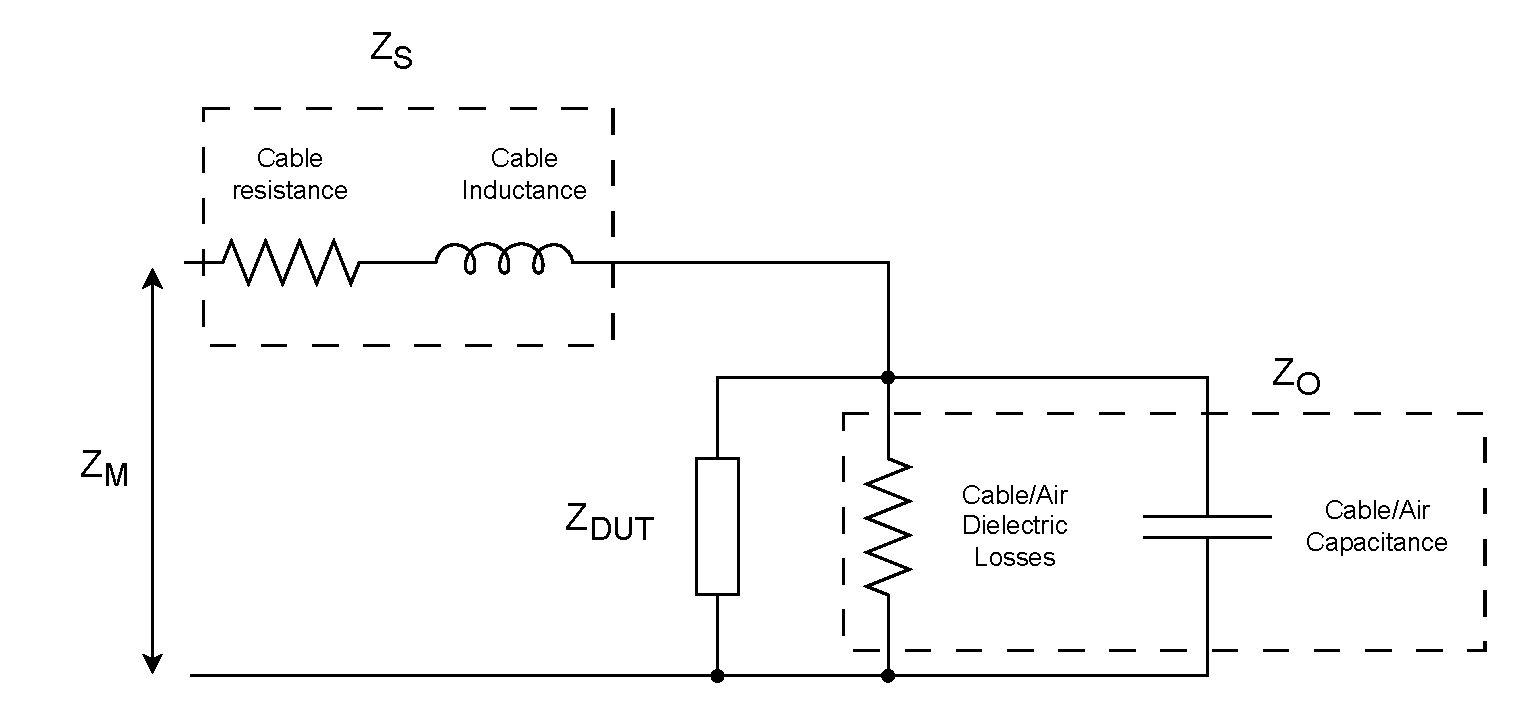
\includegraphics[clip, trim=0 0 0 0, width=1.0\textwidth]{Sections/7_SystemDesign/Figures/OpenShort.pdf}
    \caption{The measured impedance of an impedance analyzer, showing a lossy capacitor parallel to the DUT and lossy inductor in series.}
    \label{fig_7_3_3_5_OpenShort}
\end{figure}

In order to give an accurate estimate of the DUT impedance, the \textbf{short} impedance $Z_S$ and \textbf{open} impedance $Z_O$ must be known. These can however be identified by the instrument itself. If the test-terminals of the instrument are held \textbf{open}, the measured impedance can be presumed to be the open impedance $Z_O$, i.e. the impedance of the parallel capacitor and resistor. If instead the test-terminals are \textbf{shorted} the measured impedance can be assumed to be the short impedance $Z_S$, i.e. the series inductor and resistor.

By performing these measurements before any DUT is presented to the deivce, the measured impedance can be corrected to indicate what the DUT impedance is, where $Z_M$ is the measured impedance. This correction equation can be seen in equation \refq{eq:OpenShort}.

\begin{equation}
\label{eq:OpenShort}
\begin{split}
    Z_M = Z_S + \frac{Z_{DUT}Z_O}{Z_{DUT}+Z_O} \\
    \Rightarrow Z_{DUT} = -\frac{Z_O(Z_M-Z_S)}{Z_M-Z_O-Z_S} 
\end{split}
\end{equation}

This correction is then used on any measurement before it is presented to the user. 